\section{Discussion and Future work}
\label{sec:conclude}

Increased robustness in hardware has led to persistence of robots
often in hostile environments such as our oceans. The versatility of
onboard autonomy has resulted in the need to anticipate and adapt to
goals during mission execution.  Most existing autonomy approaches
fall short of dealing with the ensuing dichotomy of proactive dispatch
versus deferment.  Typically, the solution pursued is to integrate
such knowledge within the system domain description which often
results in a more complex model which is harder to maintain and
therefore likely to be error prone.  This motivates the approach to
provide an efficient solution to deduce execution policy based on the
supplementary goal information namely that of {\em urgency}.  The work
in this paper focuses on plan structure in abstraction without direct
consideration of timing constraints applied to each goal in the
plan. We are consequently able to use breadth first search within the
existing plan structure to select different execution policies for
each action within the plan. By doing so, we can improve overall
mission execution by avoiding proactivity that could lead to
inefficiency in handling new goal requests.

A number of open issues remain to be explored, however. The causal
link traversal proposed is agnostic to the temporal constraints
applied to timepoints of the plan; including such information could
greatly increase the quality of our solution.  
% When goals marked as deferred are tied to a timepoint that is
% constrained to be {\em after} a future date. 
% We need to explore this
% further in order to see how such information could be used for our
% system to automatically classify such goal as non urgent. It can also
% impact how the {\em urgent} goal propagate within the plan.
For instance, the example in Fig. \ref{fig:ex:mixed2} where consequent
to a non urgent {\em Surface} goal, planning instantiates the urgent
goal of surveying \emph{Vent1}. Currently, the policy results in
making all actions related to the non urgent {\em Surface} goal
proactive due to the proactive actions immediately \emph{following}
it.
% because it is also connected to the  urgent Survey that is constrained to be proactive
%{\em after} in the near future.
% our policy did make all the actions related to the non
% urgent goal become proactive.
This can potentially lead to premature surfacing that is then
prohibiting the agent from accepting goals in the morning. Typically
the non urgent {\em Surface}, which is to end after 13:00, is acting
as a guard on the propagation.
% Our current understanding is that this timing constraint enforcing the
% non urgent {\em Surface} to end after 1:00 is acting as a guard on the
% propagation of our heuristic.
Therefore, ideally only those actions that are directly after this
{\em Surface} goal should have been marked as proactive as shown in
Fig. \ref{fig:res:ideal}, while keeping actions preceding 13:00 deferred.
% the actions
% that are directly after this timepoint instead of continue to
% propagate to the actions leading to the surface.

\begin{figure}
  \centering
  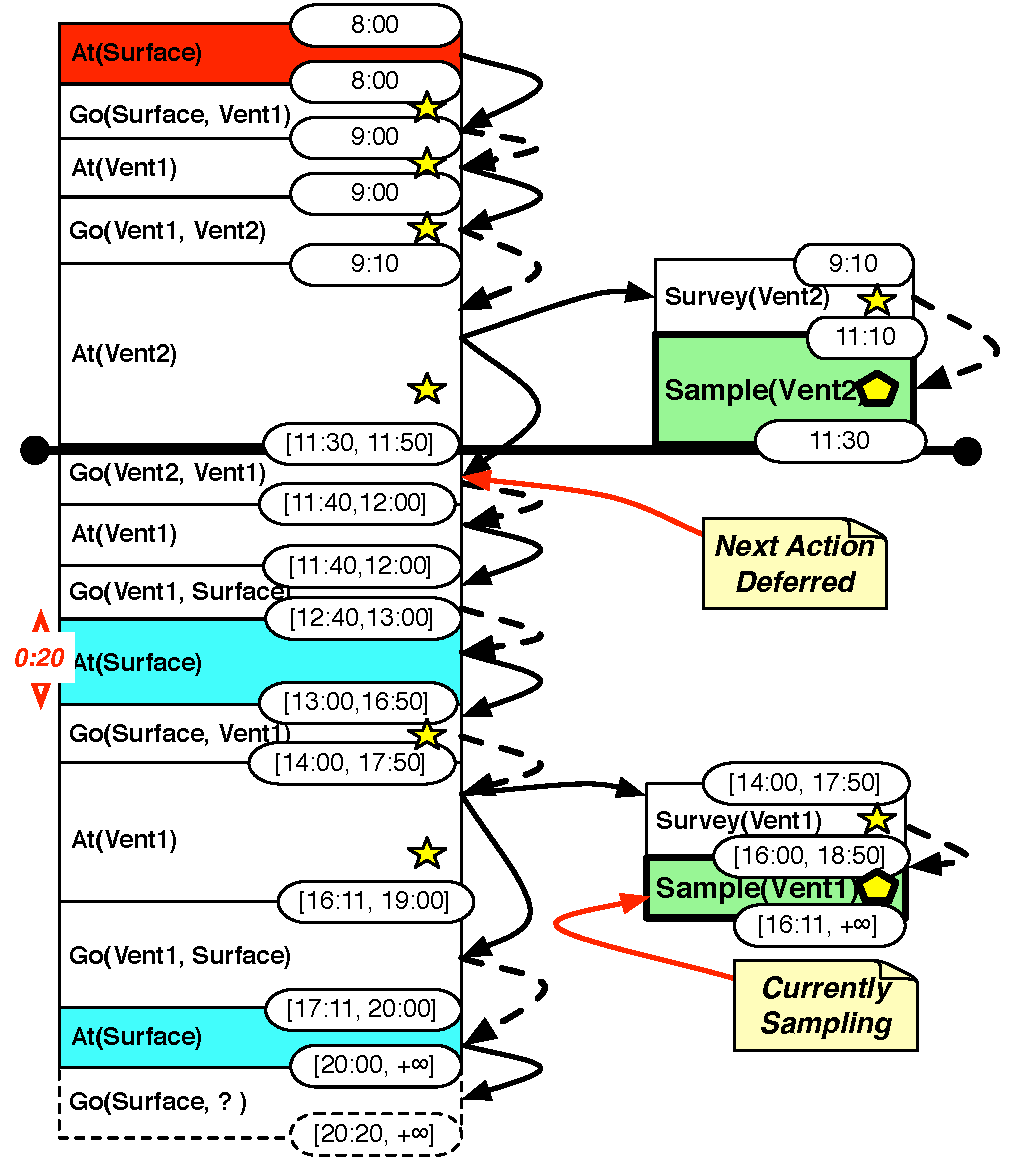
\includegraphics[width=0.7\columnwidth]{figs/example_ideal}
  \caption{\small The ideal plan solution for
    Fig. \ref{fig:ex:mixed2}. The thick line at 11:30 indicates the
    current time. Since {\em At Surface} is constrained to be at
    13:00, the AUV would be stuck for $30$ minutes.}
  \label{fig:res:ideal}
  \vskip-7mm
\end{figure}
 
Such refinement can be done only by considering the temporal
% constraints applied to plan timepoints. Should the {\em Surface} not
% have been constrained to be around 13:00 pm starting its execution
% proactively would have not blocked the vehicle at the surface. We
% plan, in the future, to explore how both the marking of the goals {\em
%   as urgent} and propagation to action can be better deduced by
% analyzing the simple temporal network (STN) supporting the current
% plan. Further, as the planner we used did not implement STNU and the
% work presented in \cite{morris01} about dynamic controllability. We
% believe that as this work is handled during planning while our
% approach is handled during plan execution, both should be easily
% complementary still the {\bf wait} actions inserted by their algorithm
% may need to be considered with a non urgent status within our
% approach.
constraints applied to the plan timepoints. Should the {\em Surface}
not have been constrained to be around 13:00 starting its execution
proactively would not have blocked the vehicle at the surface. We hope
to explore how both the marking of the goals {\em as urgent} and
propagation to action can be better deduced by analyzing the STN
supporting the current plan. The insertion of {\bf wait} actions
during planning in \cite{morris01} and the possibility of using STNUs
within our plan representation, also needs investigation with
extensions to execution time changes in plan structure.

% Further, the planner we used did
% not implement STNU or the work presented in \cite{morris01} about
% dynamic controllability. We believe that as this work is handled
% during planning while our approach is handled during plan execution
% both should be easily complementary. Still the {\bf wait} actions
% inserted by their algorithm may need to be considered with a non
% urgent status within our approach.

Such refinements are likely to improve overall execution in our agent
despite uncertainty in the number and nature of goals during mission
execution. 
% All of these refinements are considered in order to further improve
% our approach in the context of temporal planning. They would allow
% further improvement in the overall execution of our agent despite the fact
% that the set of goals it will receive is not fully known until mission 
% completion.
In our domain such a requirement is critical as our AUV is in a
dynamic environment and it is far more cost-effective to use the
limited resources (scientists and on-station time) judiciously.  The
traditional approach to such AUV surveys has been to separate
exploration and exploitation into two different surveys
\cite{Yoerger01012007}.  By improving how the vehicle handles the
inclusion of new goals, we can greatly improve the efficacy of such
surveys while generalizing to other domains.





% While there has already been work around the topic of robust
% \fcomment{This is just a quick presentation on potential future
%   direction} As we stated in the related works our approach does not
% really address dynamic controllability and has the more classic
% assumption present in many planning frameworks that time-points are
% controllable. A side effect of this is that in its current state it
% may result on the system to decide to defer action as late as
% possible. In our example, this would result on the AUV leaving Vent1
% as late as 19:00 making the rest of its plan brittle to any delay due
% for example to downward water currents on its way to the surface. This
% needs to be further addressed in the future and, especially, how our
% work can be integrated with work presented in \cite{morris01}.

% Further as of today, we consider that the qualification of the goal is
% predefined when the goal is submitted by the planner. It is possible
% though that part of this can be refined on some cases based on the
% nature of the goal. Looking back at our domain, one can note that the
% 2 goals provided are constrained differently on their start time;
% while {\em Sample Vent2} start time is limited only on its upper
% bound, the returning to surface conversely is constrained only on the
% lower bound of its start time. This difference hints on some of the
% issues we presented. While we do consider that explicit information of
% these goals help the plan execution to be improved when such
% information is not initially present. We also are aware that the
% nature of the constraints within the goal itself can help identify the
% best policy to be done. It is obvious that for Sampling Vent2 it is
% better to be proactive on the actions that contribute to this
% goal. Conversely, the other goal only matter if it appears fairly late
% in the plan which means that it is probably better to not start
% completing this part of the plan too aggressively. We plan to further
% explore how we can refine the distinction between the different
% policies by using the information provided by the constraints of the
% different objectives.
 
%%% Local Variables: 
%%% mode: latex
%%% TeX-master: "aaai13"
%%% End: 
